\documentclass[conference]{IEEEtran}
% Official IEEE layout and Times Roman body font; no margin overrides.
\usepackage[T1]{fontenc}
\usepackage{cite,graphicx,microtype,amsmath,amssymb,booktabs,array,tabularx}
\usepackage[hidelinks]{hyperref}
\interdisplaylinepenalty=2500
\newcommand{\norm}[1]{\left\lVert#1\right\rVert}
\newcommand{\diag}{\operatorname{diag}}
\newcommand{\repo}{\url{https://github.com/Marshmellow31/gps-denied-drone-navigation}}
\title{Fixed Geometric Health Decisions After LiDAR Degeneracy:\\
A Controlled Transfer Study in Two LIO Backends}
\author{\IEEEauthorblockN{Harshil Patel, Daksha Lingampeta, and Nisarg Vyas}}
\hypersetup{pdftitle={Fixed Geometric Health Decisions After LiDAR Degeneracy},
pdfauthor={Harshil Patel, Daksha Lingampeta, Nisarg Vyas}}
\begin{document}
\maketitle
\begin{abstract}
Geometric health signals describe measurement constraints, but applications
may interpret their decisions as evidence that local motion estimates have
become accurate after degeneracy. We evaluate that interpretation for fixed
policies transferred from development layouts to fresh simulated straight
corridors in FAST-LIO and Point-LIO. The revised, geometry-screened design
contains 48 matched corridor/control pairs in four length/width groups and
192 completed native runs. Each backend exposes a minimum-eigenvalue signal
and a directional DCReg detector adaptation. Scalar thresholds are selected
separately on development data and remain fixed during final evaluation.
Reference-defined recovery requires three consecutive one-second motion
windows within 0.20~m translation and $5^\circ$ rotation error. FAST-LIO
recovers in 46/48 corridor events; its scalar policy declares recovery in
14/46, with one initial false-healthy event among 46 eligible intervals.
The Point-LIO directional adaptation produces 16/47 initial false-healthy
events and declares 25/32 recoveries. Exploratory diagnosis separates misses
caused by absent raw health, failed confirmation and an already-active state
without a new declaration. These observations expose different fixed-policy
trade-offs and distinguish active health from recovery announcements. The
contribution is a reproducible transfer assessment of geometry-based decisions
against sustained motion accuracy, conditional on the screened simulation design.
\end{abstract}
\begin{IEEEkeywords}
LiDAR-inertial odometry, geometric degeneracy, recovery assessment,
diagnostic reliability, threshold transfer.
\end{IEEEkeywords}

\section{Introduction}
LiDAR-inertial odometry (LIO) estimates motion from range and inertial
measurements when global positioning is unavailable. Existing estimators
such as FAST-LIO2~\cite{fastlio} and Point-LIO~\cite{pointlio} provide motion
estimates under varied operating conditions. In a long corridor, however,
many measurements constrain lateral or vertical motion more strongly than
translation along the corridor. A diagnostic describing these geometric
constraints can inform an application, but its operational meaning requires
careful evaluation.

Three quantities must be distinguished: measurement geometry, short-window
motion accuracy, and accumulated pose drift. New visible structure may
improve current constraints without erasing an earlier position error.
Conversely, a conservative geometric rule can continue rejecting health
while measured local motion already meets a specified accuracy criterion.
Neither possibility alone is a new theoretical result. The empirical
question is how often fixed decisions agree with the accuracy claim an
application intends to make, after calibration is transferred to new layouts.

Prior work already investigates localizability, degeneracy mitigation and
recovery. OCE evaluates diagnostic agreement with ground-truth motion
usability and includes recovery behavior~\cite{oce}; DCReg characterizes
directional ill-conditioning and provides registration mitigation~\cite{dcreg}.
Consequently, recovery timing, false reassurance and geometric dependence
cannot be claimed as newly introduced concerns. We examine a narrower
setting: unchanged development-calibrated health policies evaluated on
fresh, geometry-screened corridor dimensions in two separately instrumented
LIO measurement stages.

The study uses a controlled simulator to isolate reference motion from the
online estimators. Every selected corridor has a feature-added control,
with identical motion and serialized IMU measurements. The primary endpoints
measure premature confirmed health, new recovery declarations, detected-only
delay and diagnostic availability. An exploratory investigation then examines
the decision behavior behind misses without changing the original endpoints.

The paper makes three empirical contributions: (i) a matched two-backend evaluation
of existing diagnostic families at fixed operating points; (ii) event and
paired-error estimates with explicit geometry-level uncertainty and complete
sample accounting; and (iii) a post-result diagnosis that distinguishes
absent health from an already-active state without a new declaration.
Together, these components show why score discrimination, fixed-point health
and recovery announcements must be interpreted separately when a diagnostic
is transferred to a new geometry range. The contribution is an empirical
assessment and an auditable event-level explanation, rather than a new
estimator or diagnostic formula.

\section{Related work}
\paragraph{Geometric localizability and mitigation.}
X-ICP integrates directional localizability assessment with constrained
registration~\cite{xicp}. SuperLoc predicts alignment risk for map-based
LiDAR-inertial localization~\cite{superloc}. DCReg uses Schur complements
to characterize rotational and translational ill-conditioning and couples
this characterization with mitigation~\cite{dcreg}. These systems establish
that geometric information and its directional structure are important.
Our experiment evaluates a DCReg detector adaptation on backend-specific
measurement rows; it does not execute the complete DCReg system or reproduce
its full characterization and mitigation pipeline.

\paragraph{Usability, transitions and recovery.}
OCE derives an optimization-convergence diagnostic and evaluates motion
usability against reference data, including premature recovery and
confirmation behavior~\cite{oce}. This is the closest overlap with the
present question. Informed, Constrained, Aligned examines degeneracy-aware
registration in challenging environments and transitions~\cite{ica}.
ALIVE-LIO enhances degenerate-direction estimation using learned inertial
velocity within an ESKF framework; its revised supplement also examines binary
decision switching and short degenerate intervals~\cite{alive}. Temporal
stability itself is therefore also established prior work.
The present study measures the transfer behavior of selected fixed policies;
it does not establish that those problems were previously unrecognized.

\paragraph{Environmental variation and evaluation scope.}
AdaLIO adapts parameters to corridor-like conditions~\cite{adalio}, while
GEODE provides diverse recorded degeneracy scenarios~\cite{geode}.
Our straight-corridor simulation supplies controlled motion and analytical
reference rather than comparable real-world diversity. Table~\ref{tab:overlap}
summarizes the principal distinctions. None of these named systems was
benchmarked against our policies under a shared evaluation, so the results
cannot establish superiority over them.

\begin{table*}[t]
\caption{Scope comparison. The empirical question is fixed-policy transfer
against sustained local accuracy; the named systems were not run as
shared-input baselines.}\label{tab:overlap}
\centering\small
\begin{tabularx}{\linewidth}{@{}p{.15\linewidth}XX@{}}
\toprule Work & Established concern & Relation to this study\\\midrule
OCE & Ground-truth usability, false alarms and recovery behavior & Strong
overlap; our question concerns fixed-policy transfer in two LIO backends.\\
DCReg & Directional detection, characterization and mitigation & We evaluate
only an adapted detector on each backend's rows.\\
ICA & Degeneracy mitigation and challenging transitions & Our endpoints
concern causal decisions against sustained local accuracy.\\
X-ICP / SuperLoc & Localizability and alignment risk & Relevant foundations;
not interchangeable implemented baselines here.\\
\bottomrule
\end{tabularx}
\end{table*}

\section{Problem formulation and outcome definitions}
\subsection{Local accuracy and accumulated drift}
Let $T^r_{GB}(t)$ map comparison-body coordinates to the reference world,
and $T^e_{WB}(t)$ map that same body to the estimator world. For associated
times $t_0,t_1$, define
\begin{align}
\Delta_r&=T^r_{GB}(t_0)^{-1}T^r_{GB}(t_1),\\
\Delta_e&=T^e_{WB}(t_0)^{-1}T^e_{WB}(t_1),\\
E_{\mathrm{rel}}&=\Delta_r^{-1}\Delta_e
=\begin{bmatrix}R_{\mathrm{rel}}&p_{\mathrm{rel}}\\0&1\end{bmatrix}.
\end{align}
Translation error is $\norm{p_{\mathrm{rel}}}_2$; rotation error is
$\arccos(\operatorname{clip}((\operatorname{tr}R_{\mathrm{rel}}-1)/2,-1,1))$.
Relative error does not require a fitted world-frame alignment.
Accumulated drift is evaluated separately using a single pre-entry rigid
alignment, with unit scale and no post-exit realignment. It does not define
the primary health endpoint.

Primary windows use non-overlapping nominal integer-second boundaries.
Each boundary is associated once to the nearest valid estimator pose within
$\pm0.05$~s; ties select the earlier pose and adjacent windows share the same
associated boundary. Actual durations must lie in $[0.9,1.1]$~s. Reset-crossing
windows, missing endpoints and unavailable reference are not replaced by
zero error. Reference association and frame conversion are performed offline.

\subsection{Recovery and its retrospective timing}
The independently defined exit time $t_e$ is the prescribed body crossing of
the corridor exit plane. It is a geometric anchor, not an assertion that
observability returns instantaneously. A one-second window passes if both
translation error is at most 0.20~m and rotation error at most $5^\circ$.
These operational tolerances adapt DCReg's registration-pair success
reference~\cite{dcreg} to LIO motion windows; they are not identical metrics
or physical safety requirements.

Recovery is the first triple of consecutive passing post-exit windows whose
actual endpoints all lie by $t_e+20$~s. Onset $t_o$ is the first window's
actual start and truth confirmation $t_c$ is the third window's end.
Onset is therefore retrospective. A later failed or unavailable required
estimated-motion window defines relapse at that window's start. The primary
episode ends at the first relapse or the 20~s deadline. A completed event
without a qualifying triple is a non-recovery; crashed or incomplete runs
remain execution failures. This label does not establish that each event
previously lost accuracy before exit.

\subsection{Causal health and a new declaration}
The health state machine runs on a 10~Hz grid before and after exit. At a
decision tick it uses only the latest diagnostic record at or before that
tick, at most 0.2~s old and in the same estimator segment. A newer invalid
record cannot be bypassed to reuse an older healthy value. Three distinct
healthy source records on consecutive ticks produce a transition into
confirmed health. Unhealthy, unavailable or cross-segment evidence clears
confirmation. Persistent health emits no repeated transition.

Initial false-healthy means confirmed health is active in the post-exit interval
before $t_o$, or before the deadline if no recovery occurs. Its conditional
denominator includes eligible intervals containing an available decision
tick; the unconditional rate retains every non-empty initial interval.
This endpoint concerns sustained recovery and need not imply a large
instantaneous error at each premature tick.

A recovery declaration must be a new confirmed-health transition at or
after $t_o$ and before the recovery episode ends. Its delay is declaration
time minus $t_o$. An already-active state may overlap recovered motion
without generating a qualifying declaration. Such an event is a missed
\emph{declaration}, not necessarily persistent unhealthy output.
Figure~\ref{fig:timing} illustrates the distinction.

\begin{figure}[t]
\centering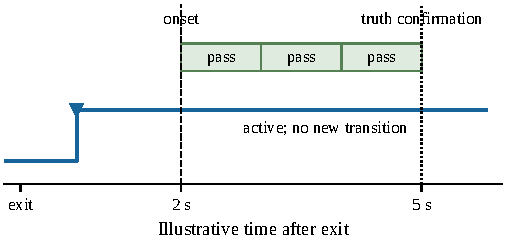
\includegraphics[width=\columnwidth]{assets/endpoint_timing.pdf}
\caption{Conceptual example, not a native result. Three passing motion windows
establish onset retrospectively. Health active before onset can persist without
a new declaration. The online policy receives no future reference windows.}\label{fig:timing}
\end{figure}

\subsection{Why active health and a declaration differ}
Let $z_j\in\{0,1\}$ be confirmed health at an available decision tick.
The notification event is
\begin{equation}
a_j=z_j(1-z_{j-1}).\label{eq:transition}
\end{equation}
If health remains active from before a recovered interval through its last
tick, every $a_j$ inside that interval is zero, although health is active
throughout. Thus a state-based permission and a new-transition notification
are different endpoints. This follows directly from the state machine; it
is not evidence that every missed declaration remains unhealthy. The
supplement provides the full argument and exact interval conventions.

\section{Diagnostic extraction and fixed policies}
\subsection{Backend-specific measurement geometry}
Read-only instrumentation records accepted point-to-plane measurement rows
without feeding reference poses to either estimator. For rows ordered as
translation then rotation, let $H=\sum_i j_i^\top j_i$ and accepted count $N$.
The normalized scalar diagnostic is
\begin{align}
G_L&=\frac{S_L H S_L}{N\,0.001},\\
S_L&=\diag(1,1,1,L^{-1},L^{-1},L^{-1}),\\
s&=\lambda_{\min}(G_{3\,\mathrm m}).
\end{align}
The 3~m lever scale and normalization are fixed protocol choices. This is
measurement geometry, excluding filter priors, rather than calibrated
posterior uncertainty. In particular, the denominator does not assert an
identical native measurement-noise weight in Point-LIO.

FAST-LIO exports the last accepted scan linearization. Point-LIO changes
state during point-time updates; its accepted groups are transported to a
common world tangent basis before pooling. For captured pre-update rotation
$R_g$, use
\begin{align}
j_{g,\mathrm{common}}&=[j_{t,g},\;j_{r,g}R_g^\top],\\
H_{\mathrm{frame}}&=\sum_g j_{g,\mathrm{common}}^\top j_{g,\mathrm{common}}.
\end{align}
Point-LIO's pooled score is not a scan-end posterior information matrix.
Each backend retains its own correspondences, poses, segments and calibration.
Frame-end output is used for the common grid; this experiment does not test
Point-LIO's maximum published output bandwidth.

\subsection{Directional detector adaptation}
For the adapted DCReg detector, reorder the raw six-dimensional Hessian
into rotation and translation blocks and calculate
\begin{align}
S_R&=H_{RR}-H_{Rt}H_{tt}^{\dagger}H_{tR},\\
S_t&=H_{tt}-H_{tR}H_{RR}^{\dagger}H_{Rt}.
\end{align}
The pseudoinverse relative rank tolerance is $10^{-12}$, an explicit
adaptation setting. Subspaces are symmetrized and checked numerically.
For each, directions with $\kappa_i=\lambda_{\max}/\lambda_i>10$ are flagged;
rank-deficient directions have explicit unbounded ratios. Raw health means
no direction is flagged. This retains the fixed detector rule, without
DCReg's full registration or mitigation~\cite{dcreg}.

At least six accepted rows and a finite numerically valid aggregate are
required. A valid rank-deficient matrix remains geometry evidence, possibly
with zero minimum eigenvalue. Startup, insufficient rows, invalid numerics
and resets are explicit unavailable states. Missing or unfinished frames
are not silently treated as healthy measurements.

\subsection{What a geometry score cannot guarantee}
A well-conditioned measurement matrix alone cannot bound estimation error
without assumptions on residual error. In the illustrative linear model
$y=Jx^\star+b$ with full-column-rank $J$, least squares gives
\begin{equation}
\widehat{x}-x^\star=(J^\top J)^{-1}J^\top b.\label{eq:bias}
\end{equation}
Choosing $b=Jv$ leaves the Hessian and its geometric scores unchanged but
gives error $v$, which is unrestricted without an assumption on $b$.
This standard linear counterexample motivates measuring motion accuracy
separately. It does not identify the physical cause of errors in our native
runs; the supplement states its assumptions and proof explicitly.

\subsection{Development-only scalar calibration}
Each backend selects one global scalar threshold using its own 32 formal
corridor development events, seeds 14--45. Candidates exhaust finite unique
valid scores plus an explicit no-alarm choice. Among candidates with at most
10\% conditional initial false-healthy events, maximize declaration sensitivity
and resolve ties toward the higher threshold. If no feasible positive-sensitivity
point exists, report that outcome explicitly. Controls and isolated feasibility
replays do not fit thresholds.

The locked thresholds are 166.16366016039856 for FAST-LIO and
123.80876977779258 for Point-LIO. The directional rule remains fixed.
Neither final scores nor final errors changed the thresholds. The development
ceiling is a selection constraint, not a final population reliability bound.

\section{Experimental design and statistical analysis}
\subsection{Controlled sensor input and matched scenes}
The simulator uses a right-handed, z-up world and opaque rectangular surfaces.
A room precedes and follows an axis-aligned corridor. The formal trajectory
starts at $x=-6$~m, includes rest and a smooth acceleration ramp, then cruises
at 0.8~m/s with prescribed smooth three-dimensional motion and attitude.
Each scene lasts 60~s and provides the full 20~s post-exit horizon.

The generic LiDAR has 16 elevations between $-15^\circ$ and $15^\circ$,
360 azimuth columns and 10~Hz scans with point acquisition spread over
0.1~s. Rays use their acquisition-time poses and nearest-surface intersections.
Range-noise standard deviation is 0.01~m. The IMU samples at 200~Hz;
white-noise standard deviations are 0.002~rad/s and 0.02~m/s$^2$.
Seeded initial gyro/accelerometer bias standard deviations are 0.003~rad/s
and 0.03~m/s$^2$, with random-walk increments of
0.0001~rad/s/$\sqrt{\mathrm s}$ and 0.001~m/s$^2$/$\sqrt{\mathrm s}$.
These are explicit stress settings, not calibration of a physical sensor.
Extrinsics and clocks are ideal; reflectivity and weather are not modeled.

Figure~\ref{fig:geometry} shows one recorded geometry.
The control adds partial baffles along the positive corridor wall while
preserving the open route. In the revised design the baffle count is
$\max(4,\lceil L/(2\,\mathrm m)\rceil-1)$, evenly spaced so longitudinal gaps
are at most 2~m. Paired scenes share motion, reference and byte-identical IMU.
Both backends receive matching corridor and control sensor-bag identities.

\begin{figure*}[t]
\centering
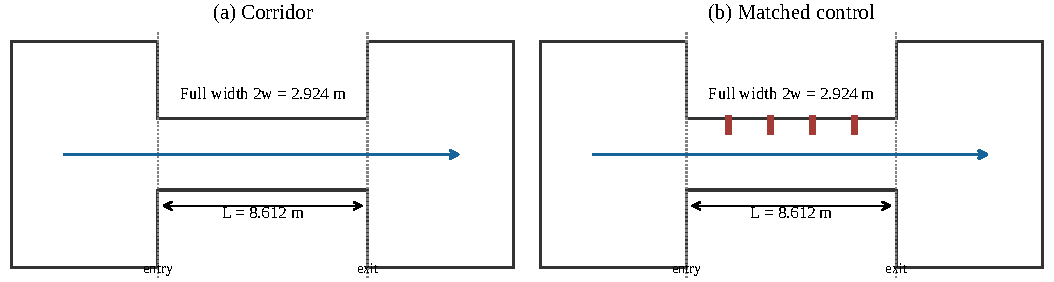
\includegraphics[width=\textwidth]{assets/geometry_schematic.pdf}
\caption{Plan-view schematic of the recorded short/narrow layout, seed 10000.
The control adds partial baffles without changing the route. Length and full
width are the saved dimensions. Walls and control spacing follow the revised
generator; the drawing omits room baffles, height, sensor rays and small
three-dimensional motion for readability. It is not a reconstruction from
estimator poses.}\label{fig:geometry}
\end{figure*}

\subsection{Development, geometry selection and exposure}
Development layouts use lengths 9--13~m and corridor half-widths
1.6--2.4~m. The fresh evaluation uses four fixed groups
(Table~\ref{tab:design}); room half-width is sampled between 4.5 and 7.5~m.
The geometry-only screen requires an axial-normal return fraction no larger
than 0.10 in the corridor, at least 0.15 in the control, and at least 0.20
in the post-exit corridor scene five seconds after exit. These are eligibility
proxies, not direct accuracy or observability labels.

\begin{table}[t]
\caption{Final geometry ranges. Width is twice the reported half-width.
Each selected geometry has corridor/control scenes and two backend runs per
scene.}\label{tab:design}
\centering\small
\begin{tabular}{@{}lrrr@{}}
\toprule Group & Length (m) & Half-width (m) & Pairs\\\midrule
Short/narrow & 8--9 & 1.3--1.5 & 12\\
Short/wide & 8--9 & 2.5--3.0 & 12\\
Long/narrow & 15--18 & 1.3--1.5 & 12\\
Long/wide & 15--18 & 2.5--3.0 & 12\\\bottomrule
\end{tabular}
\end{table}

An earlier geometry-only screen failed to supply eligible groups. A dated
protocol amendment revised control spacing and reserved fresh candidate
pools while keeping operating policies and primary outcomes fixed.
Original IDs 100--179 were excluded. The first 12 eligible fresh IDs in
ascending order within each group were selected: 48 pairs from 64 checked
candidates. Screening preceded final estimator execution. The design
therefore uses fresh instances but is not a wholly unadapted original test:
the earlier geometry screen informed the revision. An earlier screen-digest
discrepancy remains disclosed in the retained record and is not resolved by
the fresh cohort. No final accuracy or diagnostic outcome selected a geometry.

\subsection{Statistical units and uncertainty}
The final schedule contains 48 geometry clusters, two scenes and two backends,
yielding 192 native slots. Diagnostic ticks, two method rows and matched
backend outputs are not extra independent geometries. Event proportions use
95\% Wilson intervals. Group estimates retain 12 sampled geometries per group.

For the paired interior translation endpoint, planned one-second windows
lie in the central half of the corridor. Each scene contributes its median
error; each geometry contributes corridor median minus control median.
The overall estimate is the equal-weight mean of the four group means.
Uncertainty resamples paired geometry seeds within fixed groups, preserving
pairs, for 10,000 PCG64 bootstrap draws with seed 20260926; percentile
endpoints use NumPy's linear method. The analysis environment is Python
3.12.14 and NumPy 2.5.3. Intervals are conditional on these design strata.

Delay is summarized only among qualifying declarations, alongside the
detection fraction. Misses receive no invented delay and non-recovery
remains censored at the deadline. Unavailable denominators remain undefined,
not zero. The protocol requires all planned usable pairs for the complete-data
analysis; technical failures remain in the ledger and cannot be replaced
by favorable scenes. No new significance test is introduced here.

\section{Results}
\subsection{Completion and reference-defined recovery}
Both analyses completed all 48 geometry pairs and loaded 96 native scenes
per backend, for 192 completed slots. All corridor events have usable reference.
No native replay failed, and no native retry or repeat replaced a final slot.
Two operational failures remain separately recorded: Point-LIO preflight
stopped before any scene attempt because a scratch directory was absent,
and the original primary analyzer rejected extra shared-threshold metadata
before loading final reference or poses. A reviewed metadata-only adapter
resolved the latter without changing the scientific analysis source.

FAST-LIO met the recovery rule in 46/48 corridor events (95.8\%; Wilson
95\% interval 86.0--98.8\%); Point-LIO did so in 32/48 (66.7\%; 52.5--78.3\%).
There were two and sixteen non-recoveries respectively, and one relapse per
backend. These own-backend outcomes on matching inputs are descriptive;
they do not establish general estimator superiority.

\subsection{Locked diagnostic trade-offs}
Table~\ref{tab:primary} and Fig.~\ref{fig:operating} report the four fixed policies. FAST-LIO scalar
health produced one conditional initial false-healthy event in 46 eligible
intervals, but declared only 14 of 46 actual recoveries. Its directional
adaptation declared 38/46 with four premature-health events. Point-LIO scalar
declared 27/32 recoveries and produced four initial false-healthy events in
47 eligible intervals. Its directional adaptation declared 25/32 and
produced 16/47 premature-health events.

\begin{table}[t]
\caption{Locked policy outcomes. FH is conditional initial false-healthy;
declarations are among own-backend recovered events. Delay conditions on
declarations only. Unconditional FH counts are 1/48, 4/48, 4/48 and 16/48.}\label{tab:primary}
\centering\footnotesize\setlength{\tabcolsep}{2.8pt}
\begin{tabular}{@{}llrrrr@{}}
\toprule
Backend & Policy & Initial FH & Declarations & Misses & Delay (s)\\\midrule
FAST-LIO & Scalar & 1/46 & 14/46 & 32 & 0.850\\
FAST-LIO & Fixed Schur & 4/46 & 38/46 & 8 & 6.800\\
Point-LIO & Scalar & 4/47 & 27/32 & 5 & 3.400\\
Point-LIO & Fixed Schur & 16/47 & 25/32 & 7 & 3.000\\
\bottomrule
\end{tabular}

\end{table}

\begin{table*}[t]
\caption{Wilson event intervals. Policies within each backend share events;
these are not independent-proportion comparisons.}\label{tab:intervals}
\centering\small\begin{tabular}{@{}llrr@{}}
\toprule
Backend & Policy & Conditional FH (\%; 95\% CI) & Declarations (\%; 95\% CI)\\\midrule
FAST-LIO & Scalar & 2.2 [0.4, 11.3] & 30.4 [19.1, 44.8]\\
FAST-LIO & Fixed Schur & 8.7 [3.4, 20.3] & 82.6 [69.3, 90.9]\\
Point-LIO & Scalar & 8.5 [3.4, 19.9] & 84.4 [68.2, 93.1]\\
Point-LIO & Fixed Schur & 34.0 [22.2, 48.3] & 78.1 [61.2, 89.0]\\
\bottomrule
\end{tabular}

\end{table*}

All four policies have 9,600/9,600 available decision ticks in the primary
post-exit horizon. This does not imply correct decisions or guarantee a
tick in an extremely short initial unrecovered interval; hence the conditional
FH denominators of 46 and 47 differ from 48. Scalar FH upper confidence
bounds exceed the development ceiling of 10\%; the final sample establishes
no population guarantee below that ceiling. FAST-LIO scalar's 0.850~s
median delay conditions on just 14 declarations, with 32 missed recoveries.
It cannot be interpreted as superior overall responsiveness.

\begin{figure*}[t]
\centering
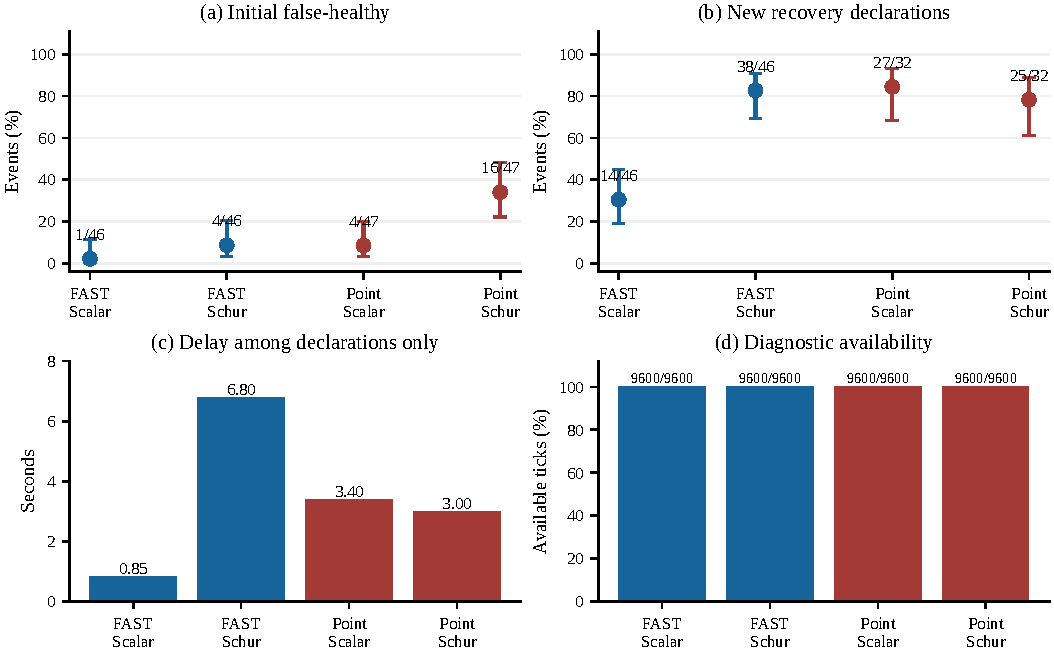
\includegraphics[width=\textwidth]{assets/operating_points.pdf}
\caption{The four locked policies: event rates with Wilson 95\% intervals,
detected-only delay, and diagnostic availability. FAST scalar declares only
14/46 recoveries despite its short conditional delay. Full score availability
is not equivalent to reliable health decisions.}\label{fig:operating}
\end{figure*}

\subsection{Geometry groups and paired interior error}
Table~\ref{tab:groups} retains the full recovery denominators. Point-LIO
recovered in 24/24 narrow versus 8/24 wide corridors. Its four scalar
initial false-healthy events occurred in long/narrow layouts (4/12), while
FAST-LIO scalar declared only 1/12 long/wide recoveries. Four-group summaries
were predeclared; emphasizing these particular patterns afterward is
exploratory, and no causal width effect is established.

\begin{table}[t]
\caption{Own-backend recovery under the fixed rule. Each group has 12 shared
input geometries. One FAST-LIO long/wide and one Point-LIO short/wide event
later relapse.}\label{tab:groups}
\centering\footnotesize
\begin{tabular}{@{}lrrrr@{}}
\toprule & \multicolumn{2}{c}{FAST-LIO} & \multicolumn{2}{c}{Point-LIO}\\
Group & Rec. & NR & Rec. & NR\\\midrule
Short/narrow & 12/12 & 0 & 12/12 & 0\\
Short/wide & 10/12 & 2 & 4/12 & 8\\
Long/narrow & 12/12 & 0 & 12/12 & 0\\
Long/wide & 12/12 & 0 & 4/12 & 8\\\bottomrule
\end{tabular}
\end{table}

The equal-group mean corridor-minus-control interior translation difference
was +0.194~m [0.086, 0.311] for FAST-LIO and +0.149~m [0.068, 0.230] for
Point-LIO (geometry-bootstrap 95\% intervals). Positive aggregate effects
do not establish a uniform benefit from control features: Point-LIO's
short/narrow group mean was $-0.087$~m. The separate backend intervals are
not a between-estimator superiority test. Relapse endpoints have only one
event per backend; Point-LIO fixed Schur remains falsely healthy after that
relapse (1/1), while the other policies have 0/1. These samples cannot
support general relapse-reliability conclusions.

\begin{figure*}[t]
\centering
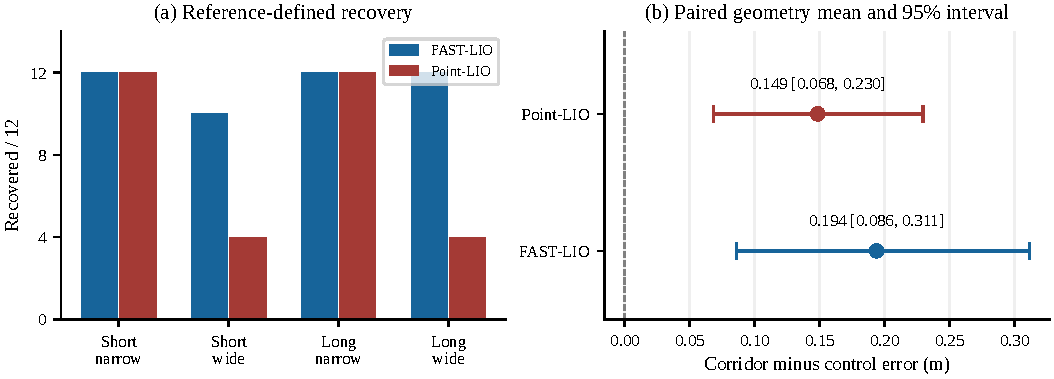
\includegraphics[width=\textwidth]{assets/geometry_effects.pdf}
\caption{(a) Recovery counts in all four fixed groups; 12 shared geometries per
group. (b) Paired interior translation-error differences with the saved
stratified geometry-bootstrap 95\% intervals. The separate backend intervals
are not a direct between-estimator comparison.}\label{fig:geometry_effect}
\end{figure*}

\subsection{Score discrimination and label sensitivity}
A high threshold-free score ranking does not guarantee a useful fixed-point
recovery notification. FAST scalar has event-weighted ROC-AUC 0.921
[0.865, 0.955], yet declares only 14/46 recoveries at the locked operating
point and causal confirmation rule. These measure different properties;
we do not choose a replacement threshold from final data. The supplement
reports ROC-AUC and average precision for every policy, with the already
computed 10,000-draw geometry-bootstrap intervals.

Under the predeclared half, primary and double motion-error tolerances,
FAST-LIO recovers in 44/48, 46/48 and 47/48 events, while Point-LIO recovers
in 31/48, 32/48 and 33/48. These sensitivity results retain all corridors
and do not replace the primary definition. The separate three-second
rate-window analysis and complete stratum results are supplied in the
supplement, with their different time and statistical units stated.

\section{Exploratory failure analysis and discussion}
\subsection{Different observable reasons for a missed declaration}
After the fixed analyses, an all-event investigation reused the frozen
labels and state machine on all 96 corridor events. All 192 diagnostic event
rows were reproduced without changing cutoffs or outcomes. The mutually
exclusive miss categories in Table~\ref{tab:misses} describe observable
decision behavior, not physical causes.

\begin{table}[t]
\caption{Exploratory partition of every missed declaration. Active means
health was active during some recovered time without a qualifying new transition;
continuous health throughout the interval is not required.}\label{tab:misses}
\centering\footnotesize\setlength{\tabcolsep}{3pt}
\begin{tabular}{@{}lrrrr@{}}
\toprule
Policy & No raw & No confirm. & Active & Total\\\midrule
FAST scalar & 30 & 2 & 0 & 32\\
FAST Schur & 5 & 2 & 1 & 8\\
Point scalar & 3 & 0 & 2 & 5\\
Point Schur & 2 & 0 & 5 & 7\\
\bottomrule
\end{tabular}

\end{table}

Figure~\ref{fig:native} illustrates two of these distinct behaviors.
Thirty FAST scalar misses have no raw healthy tick during the recovered
episode; two have intermittent raw health without confirmation. In contrast,
five of seven Point fixed-Schur misses involve active health without a new
transition. Treating every miss as persistent rejection would erase this
difference. A continuous-permission application and an event-notification
application require different interpretations of the same state trace.
This observation motivates endpoint selection in future studies, rather
than replacing the original endpoint with a more favorable result.

\begin{figure*}[t]
\centering
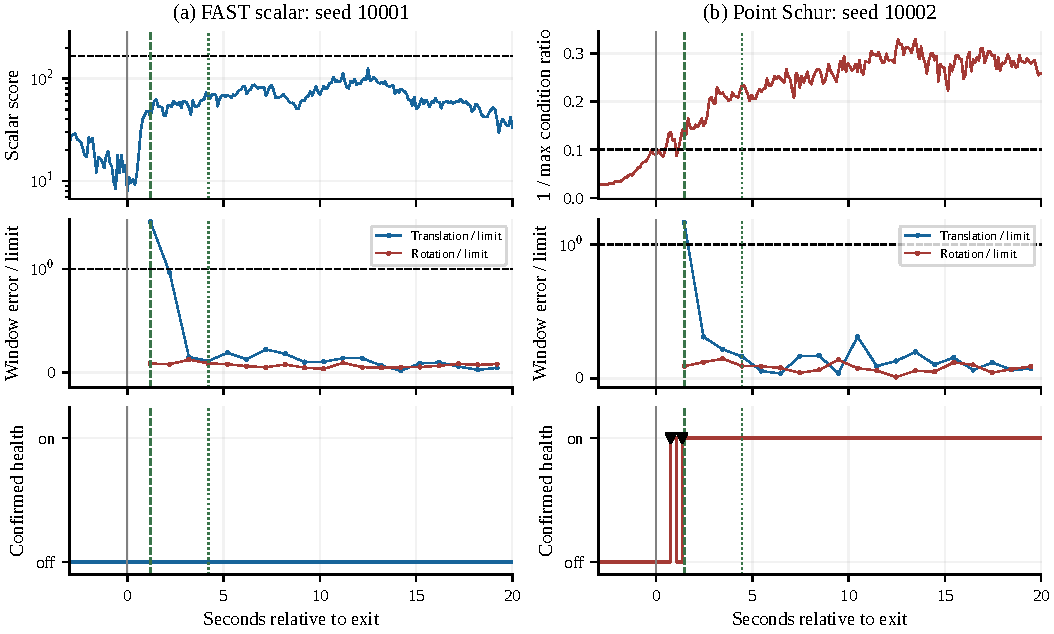
\includegraphics[width=\textwidth]{assets/native_examples.pdf}
\caption{Two native examples selected by the existing lowest-seed category
rule, not by visual appeal. Left: FAST scalar miss without a raw healthy tick
(seed 10001). Right: Point Schur miss with an already-active healthy state
(seed 10002). Green dashed/dotted lines mark retrospective onset/confirmation;
black triangles mark new online transitions. Window errors are shown at their
actual end times and divided by the primary limits; they are not online
inputs. Thin horizontal score lines are the fixed cutoffs. These examples
illustrate the all-event partition, not its prevalence.}\label{fig:native}
\end{figure*}

\subsection{Measurement support does not supply a simple explanation}
The investigation summarized accepted rows and scalar scores per event over
the fixed post-exit horizon, then compared descriptive outcome groups.
For FAST scalar, missed and detected recovered groups had almost identical
group median accepted counts (397.50 and 397.25), but different group median
scores (65.927 and 168.790). Point non-recovery events had a group median
accepted count of 456.00, compared with 411.50 in recovered/detected events.
These summaries do not support a simple monotonic count-only explanation.
They do not rule out directional distribution, correspondence quality,
visibility, IMU biases or map-history effects. Outcome grouping and the
mechanistic questions were chosen after results and remain exploratory.

\subsection{Interpretation relative to prior work}
The findings complement existing usability and degeneracy work by
documenting how selected fixed decisions behave under a specific transfer
design. The observed trade-offs do not contradict a detector's geometric
definition: measurement constraints are not identical to the history-dependent
accuracy of an estimator. A short conditional delay, full score availability
or a low point estimate of premature health is insufficient to characterize
the complete policy. Counts, missed declarations and uncertainty must be
reported together. OCE already treats usability and recovery~\cite{oce};
our evidence should be judged for the additional insight from fixed-policy
transfer and the observed failure distinctions, rather than the introduction
of those evaluation concerns.

\section{Limitations and validity}
The quantitative evidence is conditional on eligible rectangular straight
corridors, four fixed dimension groups, a prescribed trajectory family and
recorded sensor stress settings. Ideal timing/extrinsics and simplified
opaque surfaces omit reflectivity, material and weather effects. Changing
topology, motion, noise or initialization may change the results. The
geometry screen conditions the sampled design; axial-normal coverage is
not a general observability proof. The amended controls reflect information
from a failed earlier screen, even though final estimator outcomes did not
tune the policies.

There are 48 geometry clusters and only 12 per group. The emphasized width
pattern is exploratory, and its cause has not been isolated. Each backend
has its own instrumented measurement stage, settings and pose-derived labels;
we do not infer a universal backend ranking. The directional comparator is
an adaptation, not full DCReg, and no shared comparison with OCE, X-ICP,
SuperLoc or other complete systems was run. The recovery label is a specified
post-exit accuracy condition, not proof that accuracy was first lost in
every event, and active-state usability differs from a new declaration.

Real-recording work does not close these limits. The Hilti-Oxford Exp18
development pilot had only 13/56 usable matched post-exit one-second windows
and 0/56 three-second windows; its reference was partly LiDAR-map-derived.
Earlier GEODE attempts were retained as failures. Neither supplies independent
real-world sustained-recovery evidence for this paper. No physical aircraft
was tested. Internal implementation and accounting reviews are scoped
verification, not journal peer review or scientific novelty acceptance.

\section{Conclusion}
Fixed geometric policies exhibited distinct premature-health and
missed-declaration behavior when transferred to fresh, screened corridor
layouts in FAST-LIO and Point-LIO. Low observed premature health could
coexist with many missed recoveries, while the fixed directional adaptation
could produce substantial premature health in Point-LIO. Exploratory
diagnosis showed that a missed declaration can reflect absent health,
failed confirmation or an already-active state, with different operational
implications. These controlled findings support evaluating diagnostic
decisions against the specific accuracy and notification requirement of an
application. Broader validation and a precise comparison with the closest
literature are required before extending the conclusions beyond this design.

\section*{Reproducibility and evidence availability}
The repository is \repo. Compact evidence includes the final method/group
CSVs, accepted analysis JSONs, event ledger, native receipts, figure manifests,
protocol amendments, source/configuration identities and retained workflow
failures under \texttt{research\_paper/}. The evaluated geometry-v2 inventory
binds 197 artifacts; a separately accepted metadata-compatibility supplement
preserves the original scientific analysis. The manuscript is a later
document and is not itself part of that scientific freeze.

The verified portable package is
\texttt{reproduction/lidar\_recovery\_20261023/}, recorded at repository
revision \texttt{d696dab}. It includes code, configurations, reviewed
protocols, compact results, consumed native pose/health/reference streams
and offline Python dependency installers. A relocated copy in a fresh
offline-installed environment rebuilt four numerical reports and 20 figures,
and reproduced all 96 recovery labels and 192 diagnostic event rows.
Primary-window numerical error differences were at most
$7.1\times10^{-15}$; labels and decisions matched exactly. The 197-entry
implementation gate remained enforced. Current and exact frozen test
versions are retained separately with restoration provenance.

The accompanying supplement adds exact native identities/configuration,
all 64 revised screen candidates, sensitivity/ROC/AP reporting, and all
192 policy-event rows. Machine-readable native and event ledgers retain
full precision. Raw bags, Jacobian sidecars and native binaries/environments
remain external; replaying estimators from scratch is separate from stream
reanalysis. No native experiment, threshold fitting, bootstrap rerun or new
significance test was performed for this revision.

\section*{Author and submission information}
The author names follow the existing project draft. Affiliations,
corresponding author, contribution statement, funding and competing-interest
declarations require confirmation by the human authors. AI assistance was
used in research tooling and manuscript preparation; the scope and required
disclosure must be checked against the selected venue. All scientific
claims and references remain the responsibility of the human authors.
This working version uses the official IEEEtran conference class and its
Times Roman text typography. A selected venue may require a different mode,
page budget or anonymity treatment. It has not been submitted for peer review.

\begin{thebibliography}{10}
\bibitem{fastlio} W. Xu, Y. Cai, D. He, J. Lin, and F. Zhang,
``FAST-LIO2: Fast Direct LiDAR-inertial Odometry,'' 2021.
\url{https://arxiv.org/abs/2107.06829}.
\bibitem{pointlio} D. He, W. Xu, N. Chen, F. Kong, C. Yuan, and F. Zhang,
``Point-LIO: Robust High-Bandwidth Light Detection and Ranging Inertial
Odometry,'' \emph{Advanced Intelligent Systems}, vol. 5, no. 7,
article 2200459, 2023. \url{https://doi.org/10.1002/aisy.202200459}.
\bibitem{oce} J. Zhang, M. Zhu, C. Sun, F. Guo, Q. Zhan, and R. Shen,
``OCE: an optimization convergence metric for LiDAR SLAM degeneracy
detection,'' \emph{Autonomous Intelligent Systems}, vol. 6, article 21,
2026. \url{https://doi.org/10.1007/s43684-026-00144-1}.
\bibitem{dcreg} X. Hu, X. Chen, M. Jia, J. Wu, P. Tan, and S. L. Waslander,
``DCReg: Decoupled Characterization for Efficient Degenerate LiDAR
Registration,'' arXiv:2509.06285v3, 2026.
\url{https://arxiv.org/abs/2509.06285v3}.
\bibitem{xicp} T. Tuna, J. Nubert, Y. Nava, S. Khattak, and M. Hutter,
``X-ICP: Localizability-Aware LiDAR Registration for Robust Localization in
Extreme Environments,'' arXiv:2211.16335v4, 2024.
\url{https://arxiv.org/abs/2211.16335v4}.
\bibitem{superloc} S. Zhao et al., ``SuperLoc: The Key to Robust
LiDAR-Inertial Localization Lies in Predicting Alignment Risks,''
arXiv:2412.02901v2, 2025. \url{https://arxiv.org/abs/2412.02901v2}.
\bibitem{ica} T. Tuna, J. Nubert, P. Pfreundschuh, C. Cadena,
S. Khattak, and M. Hutter, ``Informed, Constrained, Aligned: A Field
Analysis on Degeneracy-aware Point Cloud Registration in the Wild,''
arXiv:2408.11809v3, 2025. \url{https://arxiv.org/abs/2408.11809v3}.
\bibitem{alive} S. Kim, D. Lee, J. Hong, S. Park, H. Jo, and S. Han,
``ALIVE-LIO: Degeneracy-Aware Learning of Inertial Velocity for Enhancing
ESKF-Based LiDAR-Inertial Odometry,'' arXiv:2604.02706v2, 2026.
\url{https://arxiv.org/abs/2604.02706v2}.
\bibitem{adalio} H. Lim, D. Kim, B. Kim, and H. Myung,
``AdaLIO: Robust Adaptive LiDAR-Inertial Odometry in Degenerate Indoor
Environments,'' arXiv:2304.12577v1, 2023.
\url{https://arxiv.org/abs/2304.12577v1}.
\bibitem{geode} Z. Chen et al., ``Heterogeneous LiDAR Dataset for
Benchmarking Robust Localization in Diverse Degenerate Scenarios,''
arXiv:2409.04961v2, 2024. \url{https://arxiv.org/abs/2409.04961v2}.
\end{thebibliography}
\end{document}
